%
% File acl2015.tex
%
% Contact: car@ir.hit.edu.cn, gdzhou@suda.edu.cn
%%
%% Based on the style files for ACL-2014, which were, in turn,
%% Based on the style files for ACL-2013, which were, in turn,
%% Based on the style files for ACL-2012, which were, in turn,
%% based on the style files for ACL-2011, which were, in turn, 
%% based on the style files for ACL-2010, which were, in turn, 
%% based on the style files for ACL-IJCNLP-2009, which were, in turn,
%% based on the style files for EACL-2009 and IJCNLP-2008...

%% Based on the style files for EACL 2006 by 
%%e.agirre@ehu.es or Sergi.Balari@uab.es
%% and that of ACL 08 by Joakim Nivre and Noah Smith

\documentclass[11pt]{article}
\usepackage{acl2015}
\usepackage{times}
\usepackage{url}
\usepackage{latexsym}
\usepackage{algorithm}
\usepackage{algorithmic}
\usepackage{fullpage}
\usepackage{graphicx}
\usepackage{longtable}
\usepackage{lscape}
\usepackage{CJKutf8}
\usepackage[hyphens]{url}
\usepackage{footnote}
\begin{CJK*}{UTF8}{gbsn}
%\setlength\titlebox{5cm}

% You can expand the titlebox if you need extra space
% to show all the authors. Please do not make the titlebox
% smaller than 5cm (the original size); we will check this
% in the camera-ready version and ask you to change it back.


\title{SECOND LANGUAGE LEARNING FROM NEWS WEBSITES}

\author{First Author \\
  Affiliation / Address line 1 \\
  Affiliation / Address line 2 \\
  Affiliation / Address line 3 \\
  {\tt email@domain} \\\And
  Second Author \\
  Affiliation / Address line 1 \\
  Affiliation / Address line 2 \\
  Affiliation / Address line 3 \\
  {\tt email@domain} \\}

\date{}

\begin{document}

\maketitle
\begin{abstract}
Learning a second language is difficult and requires
constant revision and immersion.  Fortunately, many of us take the
time to update ourselves through reading news on a daily basis.  
In this final year project, we merge both of these goals into a Web browser extension that allows a reader to learn and master vocabulary items. 
We conducted a user survey to evaluate our system against user requirements collected through an earlier survey. Since we find a word's context to be useful in learning a vocabulary, we further adopt word sense disambiguation (WSD)
technique to show the best translation for each word in the context.
Our proposed WSD method, leveraging the extension of standard machine translation system, significantly betters  baseline methods in both coverage and accuracy.
\end{abstract}

% Tao: Need to highlight the research gap (e.g., the drawbacks of existing methods for CWSD) and contributions of this work
\section{Introduction}
\label{intro}

%
% The following footnote without marker is needed for the camera-ready
% version of the paper.
% Comment out the instructions (first text) and uncomment the 8 lines
% under "final paper" for your variant of English.
% 
\iffalse
\blfootnote{
    %
    % for review submission
    %
    \hspace{-0.65cm}  % space normally used by the marker
    Place licence statement here for the camera-ready version, see
    Section~\ref{licence} of the instructions for preparing a
    manuscript.
    %
    % % final paper: en-uk version (to license, a licence)
    %
    % \hspace{-0.65cm}  % space normally used by the marker
    % This work is licensed under a Creative Commons 
    % Attribution 4.0 International Licence.
    % Licence details:
    % \url{http://creativecommons.org/licenses/by/4.0/}
    % 
    % % final paper: en-us version (to licence, a license)
    %
    % \hspace{-0.65cm}  % space normally used by the marker
    % This work is licenced under a Creative Commons 
    % Attribution 4.0 International License.
    % License details:
    % \url{http://creativecommons.org/licenses/by/4.0/}
}
\fi

%Formally learning a new language is time-consuming and requires learners to invest a significant
%amount of effort. A Chrome Extension, {\it WordNews}, was developed by \cite{tao2014} to allow users to pick up Chinese vocabulary while reading online news articles. WordNews makes language learning efficient and attractive by interleaving language
%learning with the daily activity of online news reading. 
%WordNews allows users to learn from real-world examples, and to learn words in context, which is required for effective learning of vocabulary \cite{Hirsch03readingcomprehension}.

% Tao: The logic of this section does flow well: 1) some paragraphs have duplicate information, and 2) the motivation and contribution of this paper is not clear. I prefer to move the literature review to a separate section since it is quite long (almost 1.5 pages).
% Tao: tried to edit (partial)

A word takes on different meanings, largely dependent on the context
in which it is used. For example, the word ``bank'' could mean ``slope
beside a body of water'', or a ``depository financial
institution''~\footnote{\url{http://wordnetweb.princeton.edu/perl/webwn?s=bank}}. Word
Sense Disambiguation (WSD) is the task of identifying the contextually
appropriate meaning of the word. WSD is often considered a
classification task, in which the classifier predicts the sense from a
possible set of senses, known as a sense inventory, given the target
word and the contextual information of the target word. Existing WSD
systems can be categorised into either data-driven supervised or
knowledge-rich approaches. Both approaches are considered to be
complementary to each other.

%The task of Word Sense Disambiguation (WSD) is the task of identifying the correct sense/meaning of a word out of possible senses defined in a sense inventory. 
Word embeddings have become a popular word representation formalism,
and many tasks can be done using word embeddings. The effectiveness of
using word embeddings has been shown in
% Tao: cite a few more papers
several NLP tasks \cite{Turian10wordrepresentations}. The goal of our
work is to apply and comprehensively compare different uses of word
embeddings, solely with respect to WSD. We perform evaluation of the
effectiveness of word embeddings on monolingual WSD tasks from
Senseval-2 (held in 2001), Senseval-3 (held in 2004), and
SemEval-2007. After which, we evaluate our approach on English--Chinese
Cross-Lingual WSD using a dataset that we constructed for %the use of
evaluating our approach on the translation task used in educational
applications for language learning. %, such as {\it  MindTheWord}{\footnote{\url{https://chrome.google.com/webstore/detail/mindtheword/fabjlaokbhaoehejcoblhahcekmogbom?hl=en}}} and {\it WordNews}~\cite{tao2014}.

%% Min: Nav too ordinary, try without it.
% The structure of this paper will be as follows: we have first reviewed related work and methods regarding WSD, next we will discuss the applications of WSD to a category of educational applications, and outlining possible future work finally in the conclusion. 

%The task of Word Sense Disambiguation (WSD) is the task of identifying the correct sense/meaning of a word out of possible senses defined in a sense inventory. Word embeddings is a popular technique in NLP in recent years, and many tasks can be done using 
%word embeddings. The effectiveness of
%using word embeddings has been shown in 
%% Tao: cite a few more papers
%several NLP tasks \cite{Turian10wordrepresentations}
%The goal of this work is to apply and compare different uses of word embeddings for WSD. We perform evaluation of the effectiveness of word embeddings on monolingual WSD tasks from Senseval-2 (held in 2001), Senseval-3 (held in 2004), and SemEval-2007. After which, we evaluate our approach on 
%English-Chinese Cross-Lingual WSD using a dataset that we constructed for the use of evaluating our approach on the translation task used in educational applications for language learning, such as MindTheWord {\footnote{\url{https://chrome.google.com/webstore/detail/mindtheword/fabjlaokbhaoehejcoblhahcekmogbom?hl=en}}} and WordNews.
%
%
%
%A word can have different meanings depending on the context in which it is used. For example, the word ``bank" could mean ``slope beside a body of water", or a ``depository financial institution"~\footnote{\url{http://wordnetweb.princeton.edu/perl/webwn?s=bank}}. Word Sense Disambiguation is the task of identifying the contextually appropriate meaning of the word. Word Sense Disambiguation can be considered a classification task, in which the classifier predicts the sense from a possible set of senses, known as a sense inventory, given the target word and the contextual information of the target word. Existing WSD systems can be categorised into either supervised or knowledge-rich approaches. Both approaches are considered to be complementary to each other. 
%
%
%Word Sense Disambiguation is a well-studied problem and there are many different methods. Existing methods can be broadly categorised into supervised approaches, where machine learning techniques are used to learn from labeled training data, and unsupervised knowledge-rich techniques, which do not rely on labeled data. Unsupervised techniques are knowledge-rich, and rely heavily on knowledge bases and thesaurus, such as WordNet. It is noted by Navigli \shortcite{Navigli09wordsense} that supervised approaches using memory-based learning and SVM approaches have worked best. 
%%For these approaches, it is common that the only knowledge used is the first sense in WordNet, which is used as a fallback if the system is unable to disambiguate the word in the test data. 
%
%Supervised approaches involve the extraction of features and then classification using machine learning. \shortcite{Zhong2010} developed an open-source WSD system, IMS, which was state-of-the-art at the time it was developed. It is a supervised-learning based WSD system, which first has to be trained using a set of training data. IMS uses three feature types, 1. individual words in the context surrounding the target word, 2. specific ordered sequences of words appearing at specified offsets from the target word, 3. Part-Of-Speech tags of the surrounding 3 words.
%
%% \begin{itemize}
%
%% 	\item  Surrounding Words\\
%% 	Surrounding words include individual words in the surrounding context. Sentence boundaries can be crossed in this feature. Stopwords, punctuation, character symbols, and numbers are discarded. 
%
%% 	\item Local Collocations\\
%% 	A collocation is an ordered sequence of words appearing in a specified offset from the target word. 11 location collocation features are used. They are $C_{-2},_{-2}$, $C_{-1},_{-1}$,
%% 	$C_{1},_{1}$, $C_{2},_{2}$, $C_{-2},_{-1}$, $C_{-1},_{1}$, $C_{1},_{2}$, $C_{-3},_{-1}$,
%% 	$C_{-2},_{1}$, $C_{-1},_{2}$, and $C_{1},_{3}$. $C_{i},_{j}$ refers to the ordered sequence of words between positions $i$ and $j$ relative to the target word. 
%
%% 	\item Part-Of-Speech (POS) tags of surrounding words\\
%% 	The POS tags of the three words to the left and right of the target word are used for disambiguation. If a word in the window is not in the same sentence, its POS tag will be assigned as null. %The default POS tagger in the OpenNLP toolkit~\footnote{\url{http://opennlp.apache.org/}} is used.
%% \end{itemize} 
%
%Each of the features are binary features, and IMS trains a model for each word. IMS then uses an SVM for classification. IMS is open-source, provides state-of-the-art performance at the time of its publication, and is easy to extend. As such, our proposed approach focuses heavily on IMS. 
%
%Training data is required to train IMS, which is a supervised system. 
%An example of training data for training WSD system is the One-Million Sense-Tagged Instances \cite{taghipour2015one}. This is the largest dataset we know of for training WSD systems, and we make use of it for training our systems for the All-Words tasks. 
%
%WSD systems can be evaluated using either fine-grained scoring or coarse-grained scoring. In fine-grained scoring, every sense is equally distinct from each other, and answers must exactly match. In coarse-grained scoring, similar senses are grouped and treated as a single sense. A main bottleneck to Word Sense Disambiguation is the granularity of senses. Since word senses are subjective, and the boundaries between each sense is not always well-defined, an important measure for any task is the inter-annotator agreement. The inter-annotator agreement is considered the upper bound of a task. 
%
%A problem of Word Sense Disambiguation is that the granularity of senses are subjective and may not be well-defined. WordNet is a fine-grained resource, and even human annotators have trouble distinguishing between different senses of a word \cite{edmonds2002introduction}. 
%%In some WSD tasks during Senseval, coarse-grained scoring was done in order to deal with this problem. In these evaluations, similar senses of a word are clustered together and are considered to be the same sense. 
%
%Cross-Lingual WSD was partially conceived as a further attempt to solve this issue. In Cross-Lingual WSD, the specificity of a sense is determined by its correct translation. The sense inventory is the possible translations of each word in another language. Two instances are said to have the same sense if they map to the same translation in that language. In SemEval-2010~\footnote{\url{http://stel.ub.edu/semeval2010-coref/}}, a task for Cross-Lingual WSD was introduced. SemEval-2013~\footnote{\url{https://www.cs.york.ac.uk/semeval-2013/}} featured the second iteration of this task. These tasks were tasks in which an English noun were the targeted words, and the word senses were the translations in Dutch, French, Italian, Spanish and German. 
%
%
%Traditional WSD approaches are used in Cross-Lingual WSD, although some approaches make use of Statistical Machine Translation methods and features from translation. Cross-Lingual WSD involves training by making use of parallel or multilingual corpora. In the Cross-Lingual WSD task in SemEval-2013, the top approaches used a classification approach or a statistical machine translation approach. 
%
%In NLP, words can be represented in a vector space model. Traditionally, this has been done with {\it one-hot} binary vectors, where there is only one non-zero value in a high-dimensional vector. In this encoding, each dimension represents the presence of a word, and the number of dimensions of the vector space is the size of the vocabulary. In one-hot encoding, all words are considered to be independent of each other. A problem with one-hot encoding is that the large number of dimensions makes machine learning vulnerable to over-fitting. There is no notion of word similarity and all words are independent of each other. A distributed representation of words, such as word embeddings, resolves these problems by encoding words into a low dimensional space. In word embeddings, information about a word is distributed across multiple dimensions, and similar words are expected to be close to each other. Examples of word embeddings are Continuous Bag of Words \cite{mikolovword2vec}, Collobert \& Weston's Embeddings \cite{collobert2008unified}, and GLoVe \cite{pennington2014glove}. We implemented and evaluated the use of word embedding features using these embeddings in IMS. 
%
%
%An unsupervised approach using word embeddings for WSD is described by Chen \shortcite{chen2014}. This uses a model for finding representation of senses, rather than just for words, initialised using WordNet's glosses of senses. These sense vectors can then be used during Word Sense Disambiguation. A context vector can be computed by taking the average of the words in a sentence. For disambiguating a single word, the sense with the sense vector that gives maximum Cosine Similarity with this context vector is chosen as the result for disambiguation. Chen {\it et al.} gives an algorithm to disambiguate words starting from the words with fewer senses first. 
%
%A different approach is to work on extending existing WSD systems. Turian \shortcite{Turian10wordrepresentations} suggests that for any existing supervised NLP system, a general way of improving accuracy would be to use unsupervised word representations as additional features. Taghipour \shortcite{Taghipour15} used C\&W embeddings as a starting point and implemented word embeddings as a feature type in IMS. For a specified window, vectors for the surrounding words in the windows, excluding the target word, are obtained from the embeddings and are concatenated, producing $d * (w-1)$ features, where $d$ is the number of dimensions of the vector, and w is the window size. Each feature is a floating point number, which is the value of the vector in a dimension. We note that \cite{Taghipour15} only reported results for C\&W embeddings, and did not experiment on other types of word embeddings.  
%
%Other supervised approaches using word embeddings include AutoExtend \cite{rothe2015autoextend}, which extended word embeddings to create embeddings for synsets and lexemes. In their work, they also extended IMS, but used their own embeddings. Three feature types were introduced by this work, which has some similarities to how Taghipour used word embeddings, but without Taghipour's method of scaling each dimension of the word embeddings. \\
%
%
%% Apart from reviewing work on WSD, we can generalise WSD as a classification problem and look at other approaches to perform classification. We therefore experiment with the approach of using a Neural Network for classification. In Natural Language Processing, much work has been done with Recursive Neural Networks, such as Recurrent Neural Networks, and Recursive Autoencoders. These networks have shown extremely promising results in many NLP classification tasks, such as Sentiment Classification, obtaining state-of-the-art results. 
%
%The structure of this paper will be as follows: we have first reviewed related work and methods regarding WSD, next we will discuss the applications of WSD to a category of educational applications, and outlining possible future work finally in the conclusion. 




\section{Related Work}
There are many existing language learning software, which, fall into two categories, learning by  
lessons and learning vocabularies. In the first category, 
%learning in lessons, they manually design some lessons to help their 
lessons are purposefully designed to help users easily learn a foreign language.
Duolingo\footnote{\url{https://www.duolingo.com/}} is a popular websites in this category. 
For the second category
%, learning follow vocabularies, 
% Tao: "they" refers to who? Same problem for the 1st category. Edited both for you 
% they let user recite words' list or give the corresponding translations to user's input, 
users are guided to recite lists of words, or provided with a translation for their 
input word in the foreign language.
%a corresponding translation is given according to user's input.
Google Translate \footnote{\url{https://translate.google.com/}} stands out in this category. 
The service is available as desktop / mobile / web software including a chrome extension. 
We mainly compare our system  with the aforementioned two softwares.
Table~\ref{table:difference_summary} summarises important differences between 
our system and all these existing tools. Each difference serves as a motivation 
for developing our extension.

``Duolingo is a free language-learning and crowdsourced text translation 
platform''\footnote{\url{http://en.wikipedia.org/wiki/Duolingo}}.
Most people start to use Duolingo when they know a little or nothing about 
the new language. They starting from some basic lessons and improve step by step.
% Tao: your comparison is good, but you need to highlight the uniquencess of your 
% extension in introduction or some other relevant section. 
However, our target audience 
%include people who know nothing about the foreign language language as well as people 
% with a who are fairly in the foreign language.
is a mix novice and intermediate level learners of the foreign language. 
We can not only help beginners learn 
a new language but also help them continue their learning by allowing them to practice 
their foreign language. There are also a lot articles with their translations in 
Duolingo, but all the articles and their translations are manually added by 
Duolingo or users from Duolingo. Therefore, parallel articles in Duolingo are old and 
limited. However, our chrome extension is always working even for those up to the 
minute news and our user can just practice their foreign language in their daily 
readings.

\textbf{Google Translate:} ``Highlight or right-click on a section of text and click 
on Translate icon next to it to translate it to your 
language''\footnote{\url{http://en.wikipedia.org/wiki/Google_Chrome_Extensions}}. 
% Tao: please cite
Google Translate is a chrome extension that displays only the translation when user 
select a section, which can be a word, a phrase, a sentence or even a whole page. 
Our chrome extension will translate a single word only, and display the translation, 
following with the pronunciations and example sentences to help user understand and 
remember this word. Compared with our extension, Google Translate is more like an extension 
to help user understand the content of the page. Furthermore, our extension will display 
the most appropriate translation as it will refer to the context of the word.
% Tao: Not accurate. If selecting a whole sentence, Google translator also uses 
% context. You may change to ``selecting for a single word''?
% As far as I know, Google Translate will not refer to the context while 
% selecting  a single word as the selected section is the only input.

\begin{table}[ht]
  \caption{Summary of the differences}
  \label{table:difference_summary}
  \begin{center}
  \begin{tabular}{| p{2.4cm} | p{1.2cm} | p{1.2cm} |  p{1.2cm} |}
    \hline
    & Duolingo & Google Translate & Chrome Extension \\
    \hline
    Lessons & Yes & No & No \\
    \hline
    User's foreign language level & Low & Low-High & Low-High \\
    \hline
    Time consuming & Yes & No & No\\
    \hline
    Resource & Limited & Infinite & Infinite \\
    \hline
    Customizable & Yes & No & Yes \\
    \hline
    Link to External Dictionary & No & No & Yes \\
    \hline
  \end{tabular}
  \end{center}
\end{table}
\section{Algorithm}
Our extension shows the (Chinese) translation of an English word in the learning popup (see Figure~\ref{fig:software_design_4}). As we all know, one word may have multiple translations in another language, and our extension is expected to select the most appropriate one based on the context.We call such translation selection as cross-lingual word sense disambiguation (WSD).
\\
WSD is an open problem in natural language processing and ontology, aiming at identifying the proper sense of a word (i.e. meaning) in a context, when the word has multiple meanings. However, the system that I have implemented is  different from the traditional WSD. Normally, WSD is to identify its sense in its original language, but my system is to identify its sense in another language.
\\
It has been proved by a lot of studies that context is the key to learning a new language. This further suggests that a good word sense disambiguation system is necessary for our Chrome Extension. It can help user remember vocabulary efficiently and is a key feature that differentiate our software from other language learning tools.
\\
In this following, I describe four approaches that I have tried to accomplish WSD system, which is also my main progress in the second semester. The four approaches are: 
% Tao: Please give a short definition for other three methods.
\begin{itemize}
\item Frequency based: always selecting the most frequent translation (the baseline),
\item Part-of-Speech Tag based: selecting the translation based on the Part-of-Speech Tag of the English word
\item Translation based: Selecting the translation based on the result from existing Machine Translation systems
\item Category based: Selecting the translation based on the category of the news article
\end{itemize}

\subsection{Baseline}
The simplest way to select a translation from the candidates is by random. However, the correctness of this method is very low, probably less than 20\%, and is not a good baseline for other methods to compete with. Another simple idea is to always select the most commonly used translation. Luckily, when I crawled the dictionary, Google Translate does provide usage frequency of each Chinese Translation.  This turns out to be a much better result, and thus serves as a fair baseline method.
\\
\subsection{Part-of-Speech Tagger}
As we all know, many English words have more than one Part-of-Speech (POS) tags and their Chinese translations in different POS may differ a lot. For example, the word ``book" has two POS tags, noun and verb. If it is used as a noun, mostly it means a handwritten or printed work of fiction or nonfiction, which should be translated as ``书", and mostly means to reserve if used as a verb, which should be translated as ``预定". Therefore, if I can get the POS tag of the English word, it might help me identify its sense or the Chinese translation.

\begin{table}[ht]
    \caption{Sample input/output of POSTagger}
    \label{table:part_of_speech}
    \begin{center}
    \begin{tabular}{| p{5cm} | p{7cm} | p{3cm} |}
        \hline
        Input & Output & Tag Description \\
        \hline
        They are treating me like family now & They|PRP are|VBP treating|VBG me|PRP like|IN family|NN now|RB & IN | preposition or conjunction\\
        \hline
    \end{tabular}
    \end{center}
\end{table}

Among all possible on-line sources, Stanford Log-linear Part-of-Speech Tagger~\cite{Toutanova2003} is the most stable and well performed Part-of-Speech Tagger, which is developed by The Stanford Natural Language Processing Group. Column one and column two of Table~\ref{table:part_of_speech} is one sample input and output. However, the tag from Part-of-Speech Tagger is not the one we normally used. I need one more step to match the tag to its Part-of-Speech. Therefore, I followed the Part-of-Speech guidelines from the University of Pennsylvania (Penn) Treebank Tag-set. The last column of Table \ref{table:part_of_speech} is one example of the matching.

\begin{algorithm}[ht]
\caption{Part-of-Speech Tagger}
\label{algorithm:wsd_1}
\begin{algorithmic}
\REQUIRE POS Tagger, Dictionary \textless English, Chinese, POS \textgreater, Input English

\STATE{$Pairs<word,POS> \leftarrow POSTagger \leftarrow English$}

\IF{$EnglishWord \subset Dictionary.English$}
    \STATE{$TranslationList \leftarrow Dictionary.Chinese+Dictionary.POS$}
    \FOR{$word \subset Pairs.word$}
        \IF{$word = EnglishWord$}
            \STATE{$POSResult \leftarrow Pairs.POS$}
            \STATE{$Break$}
        \ENDIF
    \ENDFOR
    \FOR{$POS \subset TranslationList.POS$}
        \IF{$POS = POSResult$}
            \STATE{$FinalResult \leftarrow TranslationList.Chinese$}
            \STATE{$Break$}
        \ENDIF
    \ENDFOR
\ENDIF
\RETURN FinalResult
\end{algorithmic}
\end{algorithm}
\begin{table}[ht]
    \caption{Example input/output of POSTagger}
    \begin{tabular}{| p{2cm} | p{1.5cm} | p{5cm} | p{3.5cm} | p{2cm} |}
        \hline
        Input English & English Word & TranslationList & Pairs \textless word,POS\textgreater & FinalResult \\
        \hline
        they are treating me like family now & like & verb : 喜欢, 爱, 爱好, 待见, 好, 看上, 喜, 喜爱, 喜好 adjective : 一样, 似, 同, 相似 conjunction : 如同noun : 类 preposition : 好像, 好比, 好以 adverb : 不啻, 若 & they|PRP are|VBP treating|VBG me|PRP like|IN family|NN now|RB & 好像 \\
        \hline
    \end{tabular}
\end{table}
%\begin{figure}[ht]
%   \centering
%   \includegraphics[width=0.9\textwidth]{wsd_2.jpg}
%   \caption{Steps of using POSTagger}
%   \label{fig:wsd_2}
%\end{figure}

Algorithm \ref{algorithm:wsd_1} is the approach of using POSTagger. From Algorithm  \ref{algorithm:wsd_1}, firstly, if the word "like" need to be translated, the algorithm will fetch all the Chinese translations as well as their Part-of-Speech tag from our dictionary. Secondly, the algorithm will send the original English sentence to Part-of-Speech Tagger, which is a Java package and has been wrapped into a server. After the client has got the output from the server, it will fetch the corresponding tag and match it to Part-of-Speech tag based on the guidelines mentioned above. Lastly, it will select the translations based on the POS.
\\
In most cases, this algorithm is only a filter. There might be a few Part-of-Speech tags matched from the output and one POS tag might have a few corresponding Chinese translations. In this case, I will choose the translation with the highest frequency of use, which is actually a combination of POSTagger and baseline, so that this system is testable independently.



\subsection{Machine Translation}
Since our target is to select the most appropriate translation based on the context, using existing Machine Translation (MT) systems is also a good approach, as all of them will certainly translate words based on the context.
\\
There are mainly two kinds of MT systems. One is off-line Machine Translation systems, which are mostly not available as mostly they are build for internal usage. Luckily, NUS NLP group built one MT system before, and it has been wrapped into a server, so that I can use it as an on-line service. The other one is on-line MT system, which are wrapped as a server and open to public, such as Bing Translator or Google Translate. As only Bing Translator is free, I decide to try Bing Translator as well.
\\
The first priority of choosing a MT system is its translation quality, if it can give me a result that nearly as good as a result from human translation, then the Chinese word that I generated from the MT system will have a high chance to be correct as well. However, after I tried both MT systems, the performance of the one from NLP group is worse than Bing Translator and the server is very unstable, I decide to use Bing Translator as my Machine Translation system.
\\

\subsubsection{Bing}
\begin{table}[ht]
    \caption{Example input/output of Bing Translator}
    \label{table:bing_translator}
    \begin{tabular}{| p{7cm} | p{7cm} |}
        \hline
        Input & Output \\
        \hline
        including a 45-caliber pistol a pump shotgun and an ar-15 rifle & 包括 45 口径手枪唧筒式猎枪和 ar-15 步枪\\
        \hline
        they are asking for privacy at this time & 在这个时候他们正在寻求隐私\\
        \hline
        possessing cartridges used exclusively by the military and carrying a firearm without a license & 拥有只供军方使用的墨盒和携带火器的许可证\\
        \hline
    \end{tabular}
\end{table}
Bing Translator, also called Microsoft Translator, is a on-line Machine Translation system that developed by Microsoft team with a cloud-based API that is conveniently integrated into multiple products, tools, and solutions. Table \ref{table:bing_translator} is the sample input and output of Bing Translator.
\\
\begin{algorithm}[ht]
\caption{Bing Translator}
\label{algorithm:wsd_3}
\begin{algorithmic}
\REQUIRE Bing Translator, Dictionary \textless English, Chinese\textgreater, Input English
\STATE{$ChineseTranslation \leftarrow Bing Translator \leftarrow English$}
\IF{$EnglishWord \subset Dictionary.English$}
    \STATE{$TranslationList \leftarrow Dictionary.Chinese$}
    \STATE{$MaxLength = 0$}
    \FOR{$ChineseWord \subset TranslationList.Chinese$}
        \IF{$(ChineseWord \subset ChineseTranslation) \cap (MaxLength < ChineseWord.Length)$}
            \STATE{$FinalResult \leftarrow ChineseWord$}
        \ENDIF
    \ENDFOR
\ENDIF
\RETURN FinalResult
\end{algorithmic}
\end{algorithm}
\begin{table}[ht]
    \caption{Example input/output of Bing Translator}
    \begin{tabular}{| p{4cm} | p{1.5cm} | p{3cm} | p{3cm} | p{2cm} |}
        \hline
        Input English & English Word & Dictionary \textless English, Chinese\textgreater & ChineseTranslation & FinalResult \\
        \hline
        including a 45-caliber pistol a pump shotgun and an ar-15 rifle & pump & verb:抽, 抽水, 打气, 唧, 唧筒, 套 noun:抽水机, 唧筒 & 包括 45 口径手枪唧筒式猎枪和 ar-15 步枪 & 唧筒 \\
        \hline
    \end{tabular}
\end{table}
%\begin{figure}[ht]
%   \centering
%   \includegraphics[width=0.9\textwidth]{wsd_5.jpg}
%   \caption{Steps of using Bing Translator}
%   \label{fig:wsd_5}
%\end{figure}

Algorithm \ref{algorithm:wsd_3} is the steps of using Bing Translator. The original English sentence is ``including a 45-caliber pistol a pump shotgun and an ar-15 rifle" and ``pump" is the word that we want to translate. Firstly, this algorithm will fetch all the Chinese translations from the database. Next, it will send the original English sentence to Bing Translator using the API provided by Microsoft and get the result that returned from Bing Translator. After that, for each Chinese translation, I will check whether this translation is a substring of the Bing Translator result. If there are a few translations that can match with the Bing Translator result, I will select the longest translation. If there are a few translations with the same length and all of them can match with the Bing Translator result, I will select the translation with the highest frequency of use. In this example, both ``唧" and ``唧筒" are the substrings of Bing Translator result. As ``唧筒" have two characters and ``唧" only have one character, this algorithm will take ``唧筒" as the final result.


\subsubsection{Bing+}
\begin{table}[ht]
    \caption{Another example of Bing Translator}
    \label{table:bing_plus_1}
    \begin{tabular}{| p{4.5cm} | p{4cm} | p{1cm} | p{4.5cm} |}
        \hline
        Input & Output & Word & Dictionary\\
        \hline
        ias a result of the latest premier league broadcast rights deal all of its teams have made it into the worlds top 40 clubs & 由于最新英超联赛转播的权交易所有其团队已经进入世界顶级40名俱乐部 & top & 顶部, 顶端, 顶, 颠, 盖, 极, 尖, 尖峰, 面, 上身, 头, 上面的, 最大的, 最高的, 盖\\
        \hline
    \end{tabular}
\end{table}
Table \ref{table:bing_plus_1} is another example of Bing Translator. In this example, ``top" is the word that need to be translated. If we manually translated the word ``top" based on the Bing Translator, I would say the correct translation should be ``顶级". However, the word ``顶级" is not covered by our dictionary, so the final result generated by Bing algorithm is ``顶" as this is the only word that matches Bing Translator. Although the meaning of the word ``顶" is almost the same as that of the word ``顶级" and I, personally, would prefer to make ``顶" as one of the correct result when I tried to evaluate this example, the word ``顶级" is more accurate in this context. Therefore, is there any way to solve this problem and make the result more accurate? Yes, solving this problem requires our system to generate Chinese words that are not covered by our dictionary and the only way is to use Word Segmenter.
\\
\begin{table}[ht]
    \caption{Example of Stanford Word Segmenter}
    \label{table:bing_plus_2}
    \begin{tabular}{| p{7cm} | p{8cm} |}
        \hline
        Input & Output\\
        \hline
        问题是你将要运行直赫顿到他说的第一修正案 & 问题, 是, 你, 将要, 运行, 直赫顿, 到, 他, 说的, 第一, 修正案\\
        \hline
        博士苏斯博士知道这将是他出版的最后一本书 & 博士, 苏, 斯, 博士, 知道, 这, 将, 是, 他, 出版, 的, 最后, 一, 本, 书\\
        \hline
        进入世界顶级40名俱乐部 & 进入, 世界, 顶级, 40, 名, 俱乐部\\
        \hline
    \end{tabular}
\end{table}
\\
Text segmentation is the process of dividing written text into meaningful units, such as words, sentences, or topics. The term applies both to mental processes used by humans when reading text, and to artificial processes implemented in computers, which are the subject of natural language processing. I use Stanford Word Segmenter to do Chinese text segmentation. Stanford Word Segmenter is a open source Java package that developed by The Stanford Natural Language Processing Group. I wrapped it into a local server and Table \ref{table:bing_plus_2} contains some example of the input and output of Stanford Word Segmenter.
\\
\begin{algorithm}[ht]
\caption{Bing+}
\label{algorithm:wsd_4}
\begin{algorithmic}
\REQUIRE Bing Translator, Word Segmenter, Dictionary \textless English, Chinese\textgreater, Input English
\STATE{$ChineseTranslation \leftarrow Bing Translator \leftarrow English$}
\STATE{$SegmentedChineseTranslation \leftarrow Word Segmenter \leftarrow ChineseTranslation$}
\IF{$EnglishWord \subset Dictionary.English$}
    \STATE{$TranslationList \leftarrow Dictionary.Chinese$}
    \STATE{$MaxLength = 0$}
    \FOR{$ChineseWord \subset TranslationList.Chinese$}
        \IF{$(ChineseWord \subset ChineseTranslation) \cap (MaxLength < ChineseWord.Length)$}
            \STATE{$FinalResult \leftarrow ChineseWord$}
        \ENDIF
    \ENDFOR
    \FOR{$SegmentedWord \subset SegmentedChineseTranslation$}
        \IF{$FinalResult \subset SegmentedWord$}
            \STATE{$FinalResult \leftarrow SegmentedWord$}
        \ENDIF
    \ENDFOR
\ENDIF
\RETURN FinalResult
\end{algorithmic}
\end{algorithm}
\begin{table}[ht]
    \caption{Example input/output of Bing+}
    \begin{tabular}{| p{4cm} | p{1.5cm} | p{3cm} | p{3cm} | p{2cm} |}
        \hline
        Input English & English Word & Dictionary.Chinese & ChineseTranslation & FinalResult \\
        \hline
        as a result of the latest premier league ... have made it into the worlds top 40 clubs & top & 顶部, 顶端, 顶, 颠, 盖, 极, 尖, 尖峰, 面, 上身, 头, 上面的, 最大的, 最高的, 盖 & 由于, 最新, 英, 超联赛, 转播, 的, 权 ... 进入, 世界, 顶级, 40, 名, 俱乐部 & 顶级 \\
        \hline
    \end{tabular}
\end{table}
%\begin{figure}[ht]
%   \centering
%   \includegraphics[width=0.9\textwidth]{wsd_6.jpg}
%   \caption{Steps of Bing+}
%   \label{fig:wsd_6}
%\end{figure}
\\
Algorithm \ref{algorithm:wsd_4} is the approach of using Bing Translator together with Stanford Word Segmenter, and I would like to use Bing+ to represent this algorithm. Step one, two and three has been described in the previous section as it is exactly the same as Bing approach. From Bing approach, this algorithm will generate ``顶" as the result. After that, Bing+ approach will send the Chinese sentence returned from Bing Translator to Stanford Word Segmenter. Then, this algorithm will use the segmented word that contains the Bing result as a substring or equals to the Bing result as the final result. In this example, the final result of Bing+ is ``顶级" which is the best result that can be generated from the result of Bing Translator and also a result that does not covered by our dictionary.
\\

\subsubsection{Bing++}
\begin{table}[ht]
    \caption{Another example of Bing+ Translator}
    \label{table:bing_plus_plus_1}
    \begin{tabular}{| p{5cm} | p{5cm} | p{1cm} | p{3cm} |}
        \hline
        Input & Output after Word Segmentation & Word & Dictionary\\
        \hline
        but the world no 46 played one of his best matches crucially not crumbling when the finish line was in sight & 但, 世界, 没有, 46, 起, 最, 重要, 的, 是, 不, 崩溃, 在, 终点, 线上, 视线, 的, 时候, 他, 最, 好, 的, 比赛, 之一 & line & 线, 线路, 路线, 系, 行列, 划线于, 衲, 排, 诗句, 纹, 线条, 衬, 衲 \\
        \hline
    \end{tabular}
\end{table}
Table \ref{table:bing_plus_plus_1} is another example of Bing+ Translator. In this example, ``line" is the word that need to be translated and the correct translation based on Bing Translator should be ``线上". The Bing approach will get ``线" as the result. After the Bing approach got the result, the next step should be finding the segmented word that contains ``线" as a substring. However, both word ``线上" and word ``视线" contains word ``线" as a substring and, obviously, only the word ``线上" is the correct result and ``视线" is actually the translation for English word ``sight". As both results generated by Bing+ approach are not covered by our dictionary, the algorithm cannot get the frequency of use information. As a result, Bing+ approach will randomly choose one word, so there is only 50\% to get the correct result. Is there any way to solve this problem and always choose the correct result in this case? Yes, as long as the algorithm could get the word alignment information, it will know exactly how to match the Chinese words with those English words.
\\
\begin{table}[ht]
    \caption{Example input/output of Word Alignment}
    \label{table:bing_plus_plus_2}
    \begin{tabular}{| p{4cm} | p{3cm} | p{7.5cm} |}
        \hline
        Input & Output & Output \\
        \hline
        dr seuss knew it would be the last book he published & 博士苏斯博士知道这将是他出版的最后一本书 & 0:1|0:1 3:7|2:5 9:12|6:7 14:15|8:8 17:21|9:9 23:24|10:10 26:28|14:14 30:33|15:17 35:38|18:19 40:41|11:11 43:51|12:13 \\
        \hline
        the problem is youre going to run straight headon into the first amendment he said & 问题是你将要运行直赫顿到他说的第一修正案 & 4:10|0:1 12:13|2:2 15:19|3:3 21:28|4:5 30:32|6:7 34:41|8:8 43:48|9:10 50:53|11:11 59:63|15:16 65:73|17:19 75:76|12:12 78:81|13:13 \\
        \hline
        this is something preschoolers deal with all the time & 这是学龄前儿童处理所有的时间 & 0:3|0:0 5:16|1:1 18:29|2:6 31:39|7:8 41:43|9:10 45:47|11:11 49:52|12:13 \\
        \hline
    \end{tabular}
\end{table}
\\
Bitext word alignment or simply word alignment is the natural language processing task of identifying translation relationships among the words (or more rarely multiword units) in a bitext, resulting in a bipartite graph between the two sides of the bitext, with an arc between two words if and only if they are translations of one another. I use Bing Word Alignment API\footnote{\url{https://msdn.microsoft.com/en-us/library/dn198370.aspx}} developed by Microsoft team to get the word alignment from English to Chinese Simplified. Luckily, although this API only support very few sets of language pairs, English to Chinese Simplified is one of the few supported sets. Table \ref{table:bing_plus_plus_2} has some examples of input and output from Bing Word Alignment. The left column is the original English sentence, the column in the middle is the translated Chinese sentence and the right column is the word alignment information. For word alignment information, the colon separates start and end index, the dash separates the languages, and space separates the words. For example, in the second column, ``0:1|0:1" means the word ``dr" should match with word ``博士" and ``9:12|6:7" means the word ``knew" should match with word ``知道".

\begin{algorithm}[ht]
\caption{Bing++}
\label{algorithm:wsd_5}
\begin{algorithmic}
\REQUIRE Bing Translator, Word Segmenter, Word Alignment, Dictionary \textless English, Chinese\textgreater, Input English
\STATE{$ChineseTranslation \leftarrow Bing Translator \leftarrow English$}
\STATE{$SegmentedChineseTranslation \leftarrow Word Segmenter \leftarrow ChineseTranslation$}
\STATE{$Pair<EnglishWord,ChineseWord> \leftarrow Word Alignment \leftarrow English$}
\IF{$EnglishWord \subset Dictionary.English$}
    \STATE{$TranslationList \leftarrow Dictionary.Chinese$}
    \STATE{$MaxLength = 0$}
    \FOR{$ChineseWord \subset TranslationList.Chinese$}
        \IF{$(ChineseWord \subset ChineseTranslation) \cap (MaxLength < ChineseWord.Length)$}
            \STATE{$FinalResult_1 \leftarrow ChineseWord$}
        \ENDIF
    \ENDFOR
    \FOR{$SegmentedWord \subset SegmentedChineseTranslation$}
        \IF{$FinalResult_1 \subset SegmentedWord$}
            \STATE{$FinalResult_1 \leftarrow SegmentedWord$}
        \ENDIF
    \ENDFOR
    \FOR{$Word \subset Pairs.EnglishWord$}
        \IF{$EnglishWord = Word$}
            \STATE{$FinalResult_2 \leftarrow Pairs.ChineseWord$}
        \ENDIF
    \ENDFOR
\ENDIF
\RETURN $FinalResult_1 \cup FinalResult_2$
\end{algorithmic}
\end{algorithm}

\begin{table}[ht]
    \caption{Example input/output of Bing++}
    \begin{tabular}{| p{4cm} | p{1.2cm} | p{2.3cm} | p{3.5cm} | p{1.5cm} | p{1.5cm} |}
        \hline
        Input English & English Word & Dictionary Chinese & Chinese Translation & Bing+ & Bing++ \\
        \hline
        state department spokeswoman jen psaki said that the allies had a long history of cooperation & top & ...陈, 陈说, 称, 称述, 发表, 发言... & 国家, 部门, 的, 女, 发言人, jenpsaki, 说, 盟国, 有, 很, 长, 的, 合作, 历史 & 发言人 & 国家 \\
        \hline
    \end{tabular}
\end{table}
%\begin{figure}[ht]
%   \centering
%   \includegraphics[width=0.9\textwidth]{wsd_7.jpg}
%   \caption{Steps of Bing++}
%   \label{fig:wsd_7}
%\end{figure}


Algorithm \ref{algorithm:wsd_5} is the approach of using Bing+ approach together with the Microsoft Bing Word Alignment. First few steps are exactly the same as Bing+ approach. In this example, ``state" is the word that need to be translated. The result from Bing+ approach is ``发言人", which is the translation of ``spokeswoman", because the Chinese translation ``发言" can be translated from both ``state" and ``spokeswoman". Then step five will send the original English sentence to Bing Word Alignment. Now, there will be two final results, one from Bing+ approach and the other one from Bing Word Alignment and the algorithm will choose the correct one from these two results. In this example, ``state" will match with ``国家" and the algorithm will choose ``国家" as the final result as well.


\begin{table}[ht]
    \caption{Some examples of Bing+ and Bing++}
    \label{table:bing_plus_plus_3}
    \begin{tabular}{| p{5cm} | p{5cm} | p{2cm} | p{2cm} |}      
        \hline
        English & Chinese & Bing+ & Bing++ \\
        \hline
        oh the places youll go! rose to the bestseller list shortly after it was released in 1990 and continues to pop up there most every spring as high school and college grads transition to a new phase of life & 哦你要去的地方!升至畅销书排行榜之后不久它于1990年被释放并继续弹出那里大多数每年春天为高中和大学毕业生过渡到人生的一个新阶段 & 春天 & 年春天\\
        \hline
        the darkness of the book is what makes the optimism credible nel said & 这本书的黑暗是什么使乐观可信nel说 & 书 & 本书\\
        \hline
        other seuss books have emerged since his death in 1991 but this was the last he had a hand in & 自从他死后在1991年出现了其他苏斯博士的书,但这是他一只手在最后一次 & 最后 & 最后一次\\
        \hline
    \end{tabular}
\end{table}

One general question about this approach is that, since I can get the official word alignment from Bing Word Alignment approach, is Bing+ approach still useful? Table \ref{table:bing_plus_plus_3} contains some examples of Bing+ approach and Bing++ approach. From left to right, the four columns are original English sentence, Chinese translation, result from Bing+ approach and result from Bing++ approach. It is very obvious that the result from Bing+ approach is the substring of the result from Bing++ approach, but which one is better? As the purpose of our Word Sense Disambiguation system is to select the most appropriate translation based on the context, but Bing Translator is a bit too smart comparing with our purpose. Bing Translator will generate some Chinese words that cannot be translated from any of the English word but can make this sentence clear and smooth. In this case, our system will choose the short answer instead of the long answer. That's why in the Bing++ approach, I will keep the result both from Bing+ approach and Bing Word Alignment and choose the better one.
\\



\subsection{News Category}
The word ``interest" have two very different translations when it is used as a noun. One translation is ``the feeling of a person whose attention, concern, or curiosity is particularly engaged by something", which should be translated as ``兴趣". The other translation is ``a share, right, or title in the ownership of property, in a commercial or financial undertaking, or the like", which should be translated as ``利益". It is quite obvious that the second sense is mostly used in financial related topics. Therefore, if we can analyze the category of the original article and 
select the translation with the same category label, it might help disambiguate the word meaning.
\\
Getting the category of the original news article is very simple. Most news websites have a manually assigned a category for each news article and in most cases, the category label is part of the URL.

However, assigning a category for Chinese word is not simple. As we are dealing with news, it is good to obtain such information from Chinese news domain. I crawled 100 Chinese news articles in each category from  Baidu News\footnote{\url{http://news.baidu.com/}}, making around 1000 news articles in total. After I got all the news articles, I send all the news articles to the Stanford Chinese Word Segmenter, and further calculate word document frequency under each  category. For example, if word ``interest" is found five times in article A and three times in article B, both article A and B are under ``finance" category, then I will add two for category ``finance" of word ``interest" as it will be counted only once even it can be found multi times in one article. I will use ``weight" to represent this value and ``averageweight" is the average weight of all categories of one word. After that, I will normalize the weight and use Equation~\ref{equation:category_1} and Equation~\ref{equation:category_2} to assign categories for those Chinese words. Basically, the two equations means that, if this word can be found in at least ten different news articles and more than 80\% of the articles are under the same category, then I will use this category for this word.

\begin{equation}
averageweight > 1\\
\label{equation:category_1}
\end{equation}
\begin{equation}
threshold > 8 * averageweight\\
\label{equation:category_2}
\end{equation}

\begin{figure}[ht]
    \centering
    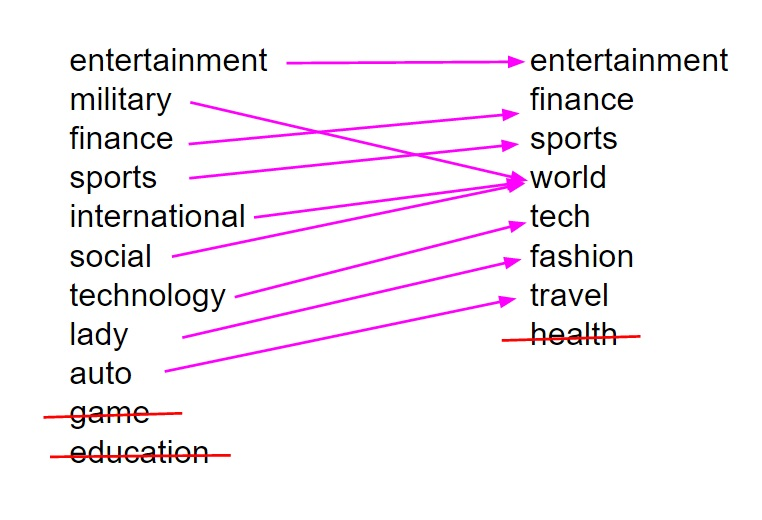
\includegraphics[width=0.9\textwidth]{wsd_4.jpg}
    \caption{Alignment between categories}
    \label{fig:wsd_4}
\end{figure}

However, the categories in Chinese and English news are not the same.
I manually aligned the categories and delete some categories when necessary.
As shown in Figure \ref{fig:wsd_4}, 
on the left side, the 11 categories are from Chinese news website and on the right side, the eight categories are from English news website. 
During the alignment, I not only take the name of category into account, but also consider the semantics of the category.
\\
\begin{algorithm}[ht]
\caption{News Category}
\label{algorithm:wsd_2}
\begin{algorithmic}
\REQUIRE Dictionary \textless English, Chinese, category\textgreater, Input English, News URL

\IF{$EnglishWord \subset Dictionary.English$}
    \STATE{$TranslationList \leftarrow Dictionary.Chinese+Dictionary.category$}
    \STATE{$EnglishCategory \leftarrow URL.category$}
    \FOR{$category \subset TranslationList.category$}
        \IF{$category = EnglishCategory$}
            \STATE{$FinalResult \leftarrow TranslationList.Chinese$}
            \STATE{$Break$}
        \ENDIF
    \ENDFOR
\ENDIF
\RETURN FinalResult

\end{algorithmic}
\end{algorithm}
\begin{table}[ht]
    \caption{Example input/output of News Cateogry}
    \begin{tabular}{| p{4cm} | p{1.5cm} | p{3cm} | p{3cm} | p{2cm} |}
        \hline
        Input English & English Word & Dictionary.Chinese & Category & FinalResult \\
        \hline
        duncan told cnns don lemon hes just painting a picture of urban street life with his lyrics & picture & ... 相, 影, 影片(entertainment), 帧, 想象, 画 ... & entertainment & 影片 \\
        \hline
    \end{tabular}
\end{table}
%\begin{figure}[ht]
%   \centering
%   \includegraphics[width=0.9\textwidth]{wsd_3.jpg}
%   \caption{Steps of using news category}
%   \label{fig:wsd_3}
%\end{figure}
\\
Algorithm \ref{algorithm:wsd_2} is the steps of using news category. The English sentence is the original sentence and ``picture" is the word that need to be translated. Firstly, the algorithm will fetch all the Chinese translations for word ``picture" and split them with comma. In this example, only the word ``影片" has a category ``entertainment". Next, the algorithm will fetch the category of the English news article from the URL, which is also ``entertainment".
In this case, the algorithm will use ``影片" as the translation for word ``picture". If a few words shares the same category, the algorithm will choose the translation with the highest frequency of use.
\section{Results}
This project has two main parts, Chrome Extension and WSD system. The Chrome Extension part is a  software development project and the best way to evaluate is to listen to users' voice. The WSD system is a standard research problem and can be evaluated with ground-truth, reporting its performance
%tested from a few very standard aspects, 
by coverage and accuracy.
\subsection{Chrome Extension}
There are a few standard aspects that can be evaluated from the Chrome Extension part, such as User Interface (UI) design, loading speed and the functionality. UI design and functionality are more related to front end, while the loading speed is highly correlated to the back end. As this project is a joint work, and I am responsible  for the front end, I limit my focus to evaluate the UI design and functionality by surveying users.
Also, as mentioned in the above chapters, we did a user requirement survey before we really start this project. From this survey, we roughly know  our potential customers' expectation and we need to check whether our Chrome Extension could satisfy them. I got 16 different responses, 15 of them are between 18 and 24, and 11 of them are professional in Chinese.
\\
For the details of the survey questions and survey results, please refer to the Appendix. In this survey, I made some screen shots of our Chrome Extension and ask subjects about their opinions. 
Most of them think that replacing some words with their corresponding Chinese translation will not influence their normal reading, but they will feel a bit uncomfortable and prefer to read the original English articles. Based on their voice, I decide to highlight the original English words as default setting instead of replacing the English words with their Chinese Translations. Besides, most subjects think our Chrome Extension is nice and would like to try it when they are going to learn a new language.
\\
\subsection{WSD System}
% Tao: 1. Why you change eval dataset?  This makes your evaluation results less convicing. I tried my best to address it. But you need to fix this problem in workshop paper. 2. You need to report the exact size of your eval dataset, e.g., # of sentences/words.
Our Word Sense Disambiguate System can be evaluated from two important aspects: coverage (i.e., is able to return a translation) and accuracy (i.e., the translation is proper). To this end, I manually annotate the ground truth. Each approach was evaluated  right after I had implemented it, therefore,  they was tested against a random but different set of recent news articles from CNN.  Though the evaluation datasets are different, it is still fair to compare their results, as the size of all dataset is sufficiently large. 


Firstly, we want our algorithm to return at least one result instead of blank. For POSTagger approach, if our dictionary do not cover the Part-of-Speech generated from Stanford POSTagger, the algorithm will return nothing. For News Category approach, as the algorithm will only assign categories for some of the Chinese translations and not all Chinese news categories can match with a English news category, so the algorithm sometimes will return nothing as well. For Bing+ and Bing++ approach, if none of the Chinese translations is the substring of the Bing result, the algorithm will return nothing. For Bing++ approach, if the word alignment information is phrase to phrase matching, for example, it may give a matching between ``in order to" and its Chinese translation, the algorithm will return nothing. Alternatively, for all the listed algorithm listed above, they can always return the translation with the highest frequency of use, but in this case, we cannot know whether the result is generated from the algorithm itself or just the baseline. That's why I choose to return a blank instead of the translation with the highest frequency of use.

\begin{table}[ht]
  \caption{Coverage for different approaches}
  \label{table:evaluation_1}
  \begin{tabular}{| p{2cm} | p{2cm} | p{2cm} |}
    \hline
     & Cover & Coverage\\
    \hline
    Baseline & 707/707 & 100\%\\
    \hline
    POSTagger & 668/707 & 94.5\%\\
    \hline
    News Category & 14/707 & 2.0\%\\
    \hline
    Bing & 555/707 & 78.5\%\\
    \hline
    Bing+ & 535/707 & 75.7\%\\
    \hline
    Bing++ & 544/707 & 76.9\%\\
    \hline
  \end{tabular}
\end{table}

Table~\ref{table:evaluation_1} contains the coverage for different approaches. As the algorithm will try to translate some word only if it is covered by our dictionary, the coverage for Baseline is always 100\%. The coverage for Bing, Bing+, Bing++ and POSTagger are roughly the same and all of them are acceptable. However, the coverage for News Category approach is only 1.9\%. One reason is that when I set the threshold for assigning categories for Chinese word, I purposely make it very high to maximize the accuracy. If the accuracy is quite high, which means this approach is quite useful, then I will lower the threshold and find the balance point.
\\
Secondly, we want our algorithm to be as accurate as possible, and the most ideal situation is that all the translation returned from the algorithm is the correct or the most appropriate translation in that context. When I evaluate the accuracy of these few approaches, I use a few news articles from CNN as the input data and manually select the most appropriate translation for all the output data. After that, I will compare the result from the algorithm and the result that I manually generated and get the accuracy.
\\
\begin{table}[ht]
  \caption{Accuracy for different approaches}
  \label{table:evaluation_3}
  \begin{tabular}{| p{2cm} | p{2cm} | p{2cm} |}
    \hline
     & Correct & Accuracy\\
    \hline
    Baseline & 405/707 & 57.3\%\\
    \hline
    POSTagger & 369/668 & 55.2\%\\
    \hline
    News Category & 1/14 & 7.1\%\\
    \hline
    Bing & 443/555 & 79.8\%\\
    \hline
    Bing+ & 433/535 & 80.9\%\\
    \hline
    Bing++ & 534/544 & 98.2\%\\
    \hline
  \end{tabular}
\end{table}
\\
Figure~\ref{table:evaluation_3} contains the accuracy of all the approaches. The last column is the accuracy for News Category approach and it is only 30\%. As mentioned in above Chapter, since the accuracy is very low, there is no need to lower the threshold and try to allocate more categories for Chinese words. The accuracy for Baseline is 69\%, which is already a fairly hight accuracy. The accuracy for Bing and POSTagger is around 69\% also, which is a bit lower than our expectation. The accuracy for Bing++ is 97\% which I think is a very good result and it is already very hard to improve. Therefore, based on my test results, Bing++ is the best approach among these five approaches.
\\

% include your own bib file like this:
%\bibliographystyle{acl}
%\bibliography{acl2015}
% use socreport.bst
\bibliographystyle{acl}
\bibliography{acl2015}

\end{document}
\clearpage\end{CJK*}